% Filename  : samplepaper.tex
% Purpose   : A sample exam paper to demonstrate how to use the 'ditpaper'
%             TeX class.
% Author    : Emmet Caulfield
% Revision  : $Id: samplepaper.tex 2 2006-02-19 20:34:45Z emmet $
% Repository: $HeadURL: http://svn.netrogen.lan/tex-ditpaper/trunk/samplepaper.tex $
%

% 'nosolution' (default) and 'solution' toggle the inclusion of solutions
% in the output. The tag --SOLUTION-OPTION--, below, is replaced by 'sed' 
% in the Makefile to cause both the paper and the solutions to be produced.
\documentclass[--SOLUTION-OPTION--]{ditpaper}

\usepackage{graphicx}
\usepackage{multirow}
\usepackage{epsf}
\usepackage{fleqn}
\usepackage[normalem]{ulem} %normalem option stop ulem from redefining the \emph command

%%%%%%%%%%%%%%%%%%%%%%%%%%%%%%%%%%%%%%%%%%%%
%% Start newcommand defs taken from aima slides style file %%%%%%%%%%%%%%
%%%%%%%%%%%%%%%%%%%%%%%%%%%%%%%%%%%%%%%%%%%%

\def\mysum{\begin{Huge}\mbox{$\Sigma$}\end{Huge}}
\def\myint{\begin{LARGE}\mbox{$\int$}\end{LARGE}}
\def\myprod{\begin{Huge}\mbox{$\Pi$}\end{Huge}}

\newcommand{\smbf}[1]{\mbox{{\smathbold #1}}}
\newcommand{\mbf}[1]{\mbox{{\bf #1}}}

%%%%%% logical symbols
\newcommand{\entails}{\models}
\newcommand{\implies}{\:\;{\Rightarrow}\:\;}
\newcommand{\textimplies}{\;{\Rightarrow}\;}
\newcommand{\impliessymbol}{\Rightarrow}
\newcommand{\lequiv}{\;\;{\Leftrightarrow}\;\;}
\newcommand{\textlequiv}{\;{\Leftrightarrow}\;}
\newcommand{\lequivsymbol}{\Leftrightarrow}
\newcommand{\xor}{\not\lequiv}
\newcommand{\All}[1]{\forall\,#1\;\;}
\newcommand{\Exi}[1]{\exists\,#1\;\;}
\newcommand{\Exii}[1]{\exists!\,#1\;\;}% -pnorvig
\newcommand{\Iot}[2]{\iota\,#1\,#2}
\newcommand{\Lam}[2]{\lambda #1\;#2}
\newcommand{\Qua}[3]{[#1\,#2\;#3]}

\newcommand{\union}{{\,{\cup}\,}}
\newcommand{\intersection}{{\,{\cap}\,}}
\renewcommand{\emptyset}{\{\,\}}
\newcommand{\emptylist}{[\,]}
\newcommand{\adjoin}[2]{\{#1|#2\}}
\newcommand{\elt}{{\,{\in}\,}}  %%%cuts down on spacing
\newcommand{\eq}{{\,{=}\,}}  %%%cuts down on spacing
\def\stimes{{\,\times\,}}       %%%cuts down on spacing

\newcommand{\sr}[1]{\mathrel{\raisebox{-0.6ex}{$\stackrel{#1}{\longrightarrow}$}}}
\newcommand{\srbox}[1]{\sr{\fboxsep=1pt\fbox{$\,{\scriptstyle #1}\,$}}}
\newcommand{\srboxbox}[1]{\sr{\fboxsep=1pt\fbox{\fbox{$\,{\scriptstyle #1}\,$}}}}

\def\Diff{\mbox{{\it Diff}}}

%%%%%% probability and decision theory
\newcommand{\pv}{\mbf{P}}
\newcommand{\qv}{\mbf{Q}}
\newcommand{\given}{\mid}
\def\transition#1#2{q(#1\rightarrow #2)}
\newcommand{\otherthan}{\overline}
\newcommand{\Parents}{Parents}
\newcommand{\parents}{parents}
\newcommand{\Children}{Children}
\newcommand{\children}{children}
\newcommand{\MarkovBlanket}{MB}
\newcommand{\markovBlanket}{mb}

\def\X{\mbf{X}}
\def\x{\mbf{x}}
\def\sx{\smbf{x}}
\def\Y{\mbf{Y}}
\def\y{\mbf{y}}
\def\sy{\smbf{y}}
\def\E{\mbf{E}}
\def\e{\mbf{e}}
\def\D{\mbf{D}}
\def\d{\mbf{d}}
\def\sbe{\smbf{e}}
\def\sE{\smbf{E}}
\def\T{\mbf{T}}
\def\O{\mbf{O}}
\def\se{\smbf{e}}
\def\Z{\mbf{Z}}
\def\z{\mbf{z}}
\def\sz{\smbf{z}}
\def\F{\mbf{F}}
\def\f{\mbf{f}}
\def\A{\mbf{A}}
\def\B{\mbf{B}}
\def\C{\mbf{C}}
\def\b{\mbf{b}}
\def\m{\mbf{m}}
\def\I{\mbf{I}}
\def\H{\mbf{H}}
\def\zeroes{\mbf{0}}
\def\ones{\mbf{1}}
\def\ev{\mbf{ev}}
\def\fv{\mbf{ev}}
\def\sv{\mbf{sv}}

%%%%%%%%%%%%%%%%%%%%%%%%%%%%%%%%%%%%%%%%%%%%
%% End newcommand defs taken from aima slides style file %%%%%%%%%%%%%%
%%%%%%%%%%%%%%%%%%%%%%%%%%%%%%%%%%%%%%%%%%%%


% These must be set or bizarre defaults will be used:
\facility{Kevin Street, Dublin 8}
\course{BSc (Hons) in Computer Science}
\examcode{S228/406}
\stage{Stage 4}
\session{Semester 2 Examinations 2009}
\title{Artificial Intelligence 2}
\examiners{Dr. John Kelleher\\
Dr. D. Lillis\\
Dr. I. Arena}
\examdate{}
\examtime{Duration: 2 Hours}
\instructions{Answer Question 1 (40 marks) \textbf{and}\par{} any 2 Other Questions (30 marks each).}

\begin{document}


% questions from across the course
\question
\begin{enumerate}
%callan
	\item Given the joint distribution for X and Y listed in Table \ref{tab:XYjoint} calculate $P(Y=y_{2})$
			\marks{5}
			\begin{answer}
			0.14 + 0.32 = 0.46
			\end{answer}
	\item Given the joint distribution for X and Y listed in Table \ref{tab:XYjoint} calculate $P(Y=y_{2} | X=x_{1})$
			\marks{5}
			\begin{answer}
			From the product rule: $P(a|b)=\frac{P(a \land b)}{P(b)}\rightarrow$\\
			$P(Y=y_{2}|X=x_{1})=\frac{P(Y=y_{2} \land X=x_{1})}{P(X=x_{1})}\rightarrow$\\
			$P(Y=y_{2}|X=x_{1})=\frac{0.14}{0.26}$
			\end{answer}
	\item In the context of machine learning, explain what is meant by \textbf{overfitting} the training data.	
		\marks{5}
		\begin{answer}
			Overfitting occurs when classifiers make decisions based on accidental properties of the training set that will lead to errors on the test set (or new data). As a result, whenever there is a large set of possible hypotheses, one has to be careful not to use the resulting freedom to find meaningless "regularity" in the data.
		\end{answer}
	\item In the context of inductive learning explain what is meant by a \textbf{consistent hypothesis}.
		\marks{5}
		\begin{answer}
		A hypothesis is consistent if it agrees with the true function on all examples that we have.
		\end{answer}
%	\item Explain what is meant by the term \textbf{abductive reasoning}.
%		\marks{5}
%		\begin{answer}
%		Abductive reasoning allows the antecedent (head) of a rule to concluded with the conclusion is true provided that doing so is consistent. Abductive reasoning is primarily diagnostic; given the effect find the likely cause.
%		\end{answer}
%\question Distinguish between \textbf{classification learning} and \textbf{regression learning}.\\
%\begin{answer}
%\begin{itemize}
%\item learning a discrete-valued function is called classification learning
%\item learning a continuous function is called regression.
%\end{itemize}
%\end{answer}
%\question Briefly describe the \textbf{performance element} of a Decision Tree.\\
%\begin{answer}
%A decision tree takes as input an object or situation described by a set of attributes and returns a �decision� � the predicted out value for the input.
%A decision tree reaches its decision by performing a sequence of tests.
%Each internal node in the tree corresponds to a test of the value of one of the properties, and the branches from the node are labeled with the possible
%values of the test.
%Each leaf node in the tree specifies the value to be returned if that leaf is reached.
%\end{answer}
\question What is the aim of \textbf{inductive logic learning}?
		\marks{5}

\begin{answer}
The aim of inductive logic learning is to find an equivalent logical expression for the goal predicate that we can use to classify examples correctly.
\end{answer}

\question In the context of inductive logic learning, what is meant by the \textbf{extension} of a hypothesis?
\marks{5}
\begin{answer}
Each hypothesis predicts that a certain set of examples, namely those that satisfy the hypotheses definition, are examples that satisfy the goal predicate. This set of examples is called the extension of the hypothesis. For example, assuming a standard interpretation, the extension of the predicate $digit(X)$ is $\{1,2,3,4,5,6,7,8,9,0\}$
\end{answer}

%\question Distinguish between the \textbf{generalisation} and \textbf{specialization} of a logical predicate.\\
%\begin{answer}
%The generalisation of a logical predicate results in the broadening of the extension of the predicate. Some of the operations that can be used to generalise a logical predicate include: converting conjunctions in the predicate to disjunctions or dropping conditions in the predicate. You would generalise a predicate in response to recognising a false negative.
%The specialisation of a logical predicate results in the narrowing of the extension of the predicate. Some of the operations that can be used to generalise a logical predicate include: converting disjunctions in the predicate to conjunctions or adding conditions in the predicate. You would specialise a predicate in response to recognising a false positive.
%\end{answer}

\item In the context of machine learning distinguish between \textbf{false negatives} and \textbf{false positives}.
\marks{5}
\begin{answer}
\begin{description}
\item [False negative] an example can be a false negative for the hypothesis, if
the hypothesis says it should be negative but in fact it is positive.
\item [False positive] an example can be a false positive for the hypothesis, if the
hypothesis says it should be positive but in fact it is negative.
\end{description}
\end{answer}


	\item In the context of machine learning, what does it mean if two classes $C_1$ and $C_2$ are described as \textbf{linearly separable}?	
		\marks{5}
		\begin{answer}
		This means that for each class $C_i$ there exists a hyperplane $H_i$ such that on its positive side lie all $x \in C_i$ and on its negative side lie all $x \in C_j , j \ne i$
		\end{answer}

\end{enumerate}

\begin{table}[t]
\caption{Joint Distribution for X and Y}
\begin{center}
\begin{tabular}{c|cc}
                  & $X=x_{1}$ & $X=x_{2}$ \\
                  \hline
$Y=y_{1}$ & 0.02        & 0.30 \\
$Y=y_{2}$ & 0.14        & 0.32\\
$Y=y_{3}$ & 0.10        & 0.12 
\end{tabular}
\end{center}
\label{tab:XYjoint}
\end{table}


\newpage

%Q2 30 marks
% reasoning under uncertainty
% aima chapters 13, 14, 15
\question
\begin{enumerate}
	%aima
	\item In your local power station, there is an alarm that senses when a temperature gauge exceeds a given threshold. The gauge measures the temperature of the core. Consider the Boolean variables $A$ (alarm sounds), $F_A$ (alarm is faulty), and $F_G$ (gauge is faulty); and multivalued nodes $G$ (gauge reading) and $T$ (actual core temperature).
	
	\begin{enumerate}
		\item Draw a Bayesian network for this domain, given that the gauge is more likely to fail when the core temperature gets too high.
		\marks{5}
		\begin{answer}
			The key aspects are: the failure nodes are parents of the sensor nodes, and the temperature node is a par ent of both the gauge and the gauge failure node. It is exactly this kind of correlation that makes it dif�cult for humans to understand what is happening in complex systems with unreliable sensors.
			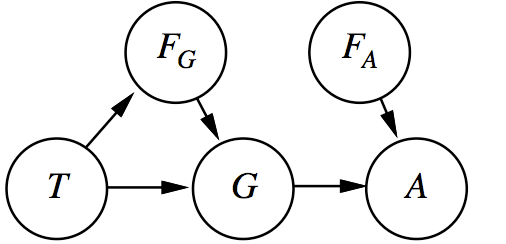
\includegraphics[width=\textwidth]{./images/nuclearpowerstationbayesiannet.png}
		\end{answer}
		\item Suppose there are just two possible actual and measured temperatures: normal and high. The probability that the gauge gives the correct temperature is $x$ when it is working, but $y$ when it is faulty. Give the conditional probability table associated with node $G$.
		\marks{5}
		\begin{answer}
			Note the semantics of $F_G$ , which is true when the gauge is faulty, i.e., not working.
			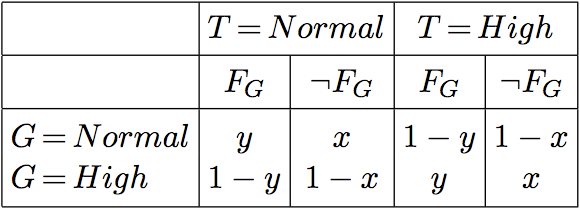
\includegraphics[width=\textwidth]{./images/cpt_node_g_q142.png}
		\end{answer}
		%\item I have left out the rest of this question fill it in when I get a chance - the CPTs for part 2 and 3 are in the images folder.
	\end{enumerate}
	
	\item Suppose you are a security guard at some secret underground installation. You want to know whether it's raining today, but your only access to the outside world occurs each morning when you see the director coming in with, or without, an umbrella. For each day $t$, the set $\textbf{E}_t$ contains a single evidence variables $U_t$ (whether the umbrella appears), and the set $\textbf{X}_t$ contains a single state variable $R_t$ (whether it is raining). Figure \ref{fig:umbrella} provides the Bayesian network structure and conditional distributions that describe this scenario. 
	\begin{enumerate}
		\item Assuming that you have a prior belief about whether it rained on day 0, just before the observation sequence begins of: $\pv(R_0) =  < 0.5 , 0.5 >$ and that the umbrella appears on day 1, so $U_1=true$, \textbf{compute the probability that it rained on day 1}, (i.e., compute $\pv(R_1|u_1)$).
		\marks{10}
		\begin{answer}
			We want to compute $\pv(R_{1}|u_{1})$. This can be computed by rewriting the general filtering model:\\
	 		$\pv(\X_{t+1}|\e_{1:t+1}) = \alpha \underbrace{\pv(\e_{t+1}|\X_{t+1})}_{Sensor~Model.}  \mysum_{x_t}  \underbrace{ \pv(\X_{t+1}|x_t)}_{Transition~Model.} \underbrace{P(x_t,|\e_{1:t})}_{Current~State~Distribution.}$\\
	 		in terms of the variables in our scenario (i.e., the hidden boolean variables $R_0, \dots, R_t$ each denoting whether or not it is raining for a particular timeslice $t=0, \dots, t$ and the evidence boolean variables $U_t, \dots U_t$ each denoting whether or not the umbrella appeared at a particular timeslice $t=0, \dots, t$). Rewriting in the filtering model in these terms give us:\\
$\pv(R_{1}|u_{1}) = \alpha \underbrace{\pv(u_{1}|R_{1})}_{Sensor~Model.}  \mysum_{r_0}  \underbrace{ \pv(R_{1}|r_0)}_{Transition~Model.} \underbrace{P(r_0)}_{Current~State~Distribution.}$\\
			Plugging in the appropriate values from the conditional probability tables give us:\\

			\begin{eqnarray*}
				\lefteqn{ \pv(R_{1}|u_{1}) = \alpha \underbrace{\langle 0.9, 0.2 \rangle}_{Sensor~Model.} \mysum_{r_0} \underbrace{ \left( \begin{array}{cc} 0.7 & 0.3 \\ 0.3 & 0.7 \\ \end{array} \right) }_{Transition~Model.} \underbrace{ \langle 0.5, 0.5 \rangle }_{Current~State~Distribution.} }\\
				& = & \alpha \underbrace{\langle 0.9, 0.2 \rangle}_{Sensor~Model.}  \underbrace{ \langle 0.7,  0.3 \rangle \times 0.5 + \langle 0.3,  0.7 \rangle \times 0.5 }_{Prediction~From~t=0~to~t=1.}\\
				& = & \alpha \underbrace{\langle 0.9, 0.2 \rangle}_{Sensor~Model.}  \underbrace{ \langle 0.5, 0.5 \rangle }_{Prediction~From~t=0~to~t=1.}\\
				& = & \alpha \langle 0.45, 0.1 \rangle \approx \langle 0.818, 0.182 \rangle
			\end{eqnarray*}
		\end{answer}
		
	\item Using the value for $\pv(R_1|u_1)$ that you computed in part (i) of this question, and assuming that the umbrella appears on day 2 (i.e. $U_2=true$), \textbf{compute the probability that it rained on day 2} (i.e., compute $\pv(R_2|u_1, u_2)$).
	\marks{10}
	\begin{answer}
	We want to compute $\pv(R_{2}|u_{1}, u_{2})$. This can be computed by rewriting the general filtering model:\\
	 $\pv(\X_{t+1}|\e_{1:t+1}) = \alpha \underbrace{\pv(\e_{t+1}|\X_{t+1})}_{Sensor~Model.}  \mysum_{x_t}  \underbrace{ \pv(\X_{t+1}|x_t)}_{Transition~Model.} \underbrace{P(x_t,|\e_{1:t})}_{Current~State~Distribution.}$\\
	 in terms of the variables in our scenario (i.e., the hidden boolean variables $R_0, \dots, R_t$ each denoting whether or not it is raining for a particular timeslice $t=0, \dots, t$ and the evidence boolean variables $U_t, \dots U_t$ each denoting whether or not the umbrella appeared at a particular timeslice $t=0, \dots, t$). Rewriting in the filtering model in these terms give us:\\
$\pv(R_2|u_1, u_2) = \alpha \underbrace{\pv(u_{2}|R_{2})}_{Sensor~Model.}  \mysum_{r_1}  \underbrace{ \pv(R_{2}|r_1)}_{Transition~Model.} \underbrace{P(r_1|u_1)}_{Current~State~Distribution.}$\\
	Plugging in the appropriate values from the conditional probability tables give us:\\

\begin{eqnarray*}
\lefteqn{ \pv(R_2|u_1, u_2) = \alpha \underbrace{\langle 0.9, 0.2 \rangle}_{Sensor~Model.} \mysum_{r_1} \underbrace{ \left( \begin{array}{cc} 0.7 & 0.3 \\ 0.3 & 0.7 \\ \end{array} \right) }_{Transition~Model.} \underbrace{ \langle 0.818, 0.182 \rangle }_{Current~State~Distribution.} }\\
& = & \alpha \underbrace{\langle 0.9, 0.2 \rangle}_{Sensor~Model.}  \underbrace{ \langle 0.7,  0.3 \rangle \times 0.818 + \langle 0.3,  0.7 \rangle \times 0.182 }_{Prediction~From~t=1~to~t=2.}\\
& = & \alpha \underbrace{\langle 0.9, 0.2 \rangle}_{Sensor~Model.}  \underbrace{  \langle 0.627, 0.373 \rangle  }_{Prediction~From~t=1~to~t=2.}\\
& = & \alpha {\langle 0.565, 0.075 \rangle} \approx \langle 0.883, 0.117 \rangle
\end{eqnarray*}
\end{answer}
\end{enumerate}

\end{enumerate}

\begin{figure}[h]
	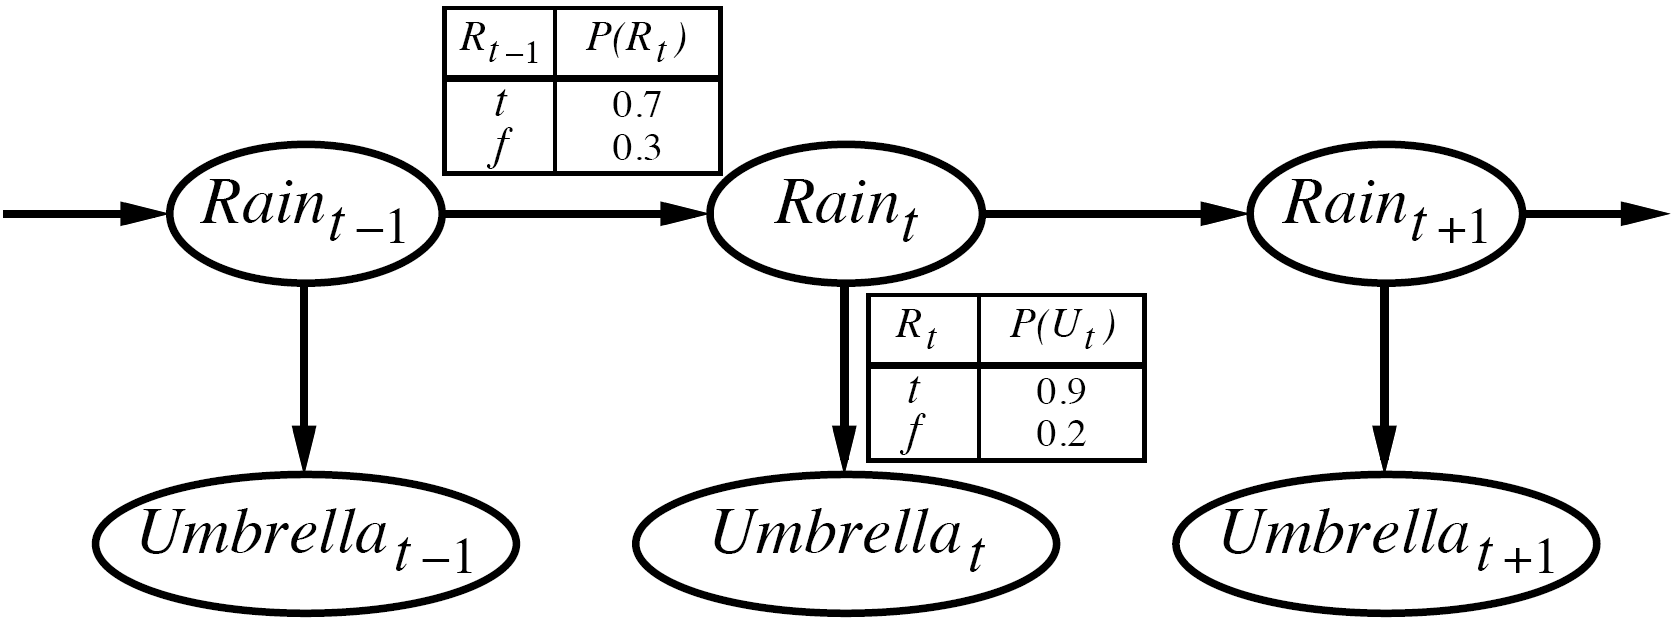
\includegraphics[width=5in]{./images/umbrella-dbn.png}
	\caption{Bayesian network structure and conditional distribution describing the umbrella world. The transition model is $P(Rain_t|Rain_{t-1})$ and the sensor model is $P(Umbrella_t|Rain_t)$}
	\label{fig:umbrella}
\end{figure}
 
\newpage

%Q3
%Inductive Learning (Decision Trees)
%aima chapters 18
\begin{table}
\begin{center}
\begin{tabular}{|c|c|c|}
$X$ & $Y$ & Class \\
\hline
T & T & + \\
T & F & - \\
T & F & + \\
T & T & + \\
F & T & - \\
\end{tabular}
\end{center}
\caption{X and Y Classification Data}
\label{tab:x-y-classification-data}
\end{table}
\question
\begin{enumerate}
\item In the context of machine learning, distinguish between \textbf{supervised} and \textbf{unsupervised} learning.
		\marks{5}
		\begin{answer}
			The distinction is that with \textbf{supervised learning} we know the actual label or category for each piece of data on which we train, whereas with \textbf{unsupervised learning} we do not know the classification of the data in the training sample. Unsupervised learning can thus often be viewed as a \textbf{clustering} task, while supervised learning can usually be seen as a \textbf{classification} task, or equivalently as a function-fitting task where one extrapolates the shape of a function based on some data points.
		\end{answer}	

\item Discuss the advantages and disadvantages of \textbf{$k$-Nearest Neighbour} classification.
				\marks{10}
				\begin{answer}
				Strengths
				\begin{enumerate}	
					\item No training involved � lazy learning
					\item New data can be added on the fly
					\item Some explanation capabilities
					\item Robust to noisy data by averaging k-nearest neighbors
				\end{enumerate}
				Weaknesses
				\begin{enumerate}
					\item Not the most powerful classification (generally its accuracy will be lower than an ANN or SVM model)
					\item Slow classification 
					\item Curse of dimensionality (as you increase the number of features you need more and more examples to cover the problem space - kNN are particularly susceptible to this issue as they do not do any feature selection).
				\end{enumerate}
			\end{answer}	

%Callan Chapter 12 Q.3
\item Table \ref{tab:x-y-classification-data} provides a classification for a data set of X Y pairs.
	\begin{enumerate}
	\item Calculate the \textbf{entropy} for this classification.
	\marks{5}
	\begin{answer}
		Entropy is $-\frac{3}{5}log_2\frac{3}{5}-\frac{2}{5}log_2\frac{2}{5}=0.971$
	\end{answer}
	\item Calculate the \textbf{information gain} for X and Y.
	\marks{10}
	\begin{answer}
		Entropy for X = T $-\frac{3}{4}log_2\frac{3}{4}-\frac{1}{4}log_2\frac{1}{4}=0.811$\\
		Entropy for X = F $0-\frac{1}{1}log_2\frac{1}{1}=0$\\
		Gain for X $0.971-(\frac{4}{5}\times0.811+\frac{1}{5}\times0)=0.322$\\
		Entropy for Y = T $-\frac{2}{3}log_2\frac{2}{3}-\frac{1}{3}log_2\frac{1}{3}=0.918$\\
		Entropy for Y = F $-\frac{1}{2}log_2\frac{1}{2}-\frac{1}{2}log_2\frac{1}{2}=1.0$\\
		Gain for Y $0.971-(\frac{3}{5}\times0.918+\frac{2}{5}\times1)=0.02$\\
	\end{answer}
	\end{enumerate}

\end{enumerate}
 
%Q4
%Neural Nets
\question 
\begin{enumerate}
\item Describe the processing stages of a McCulloch-Pits ''unit''.
\marks{10}
\begin{answer}
			The processing stages of a unit are:
			\begin{enumerate}
				\item Each unit $i$ first compute a weighted sum of its inputs:  $in_i \leftarrow \sum_j W_{j,i}  a_j$
				\item Then it applies an \textbf{activation function} $g$ to this sum to derive the output (activation) $a_i$: $a_i \leftarrow g(in_i) = g\left(\sum_j W_{j,i} a_j\right)$
			\end{enumerate}

			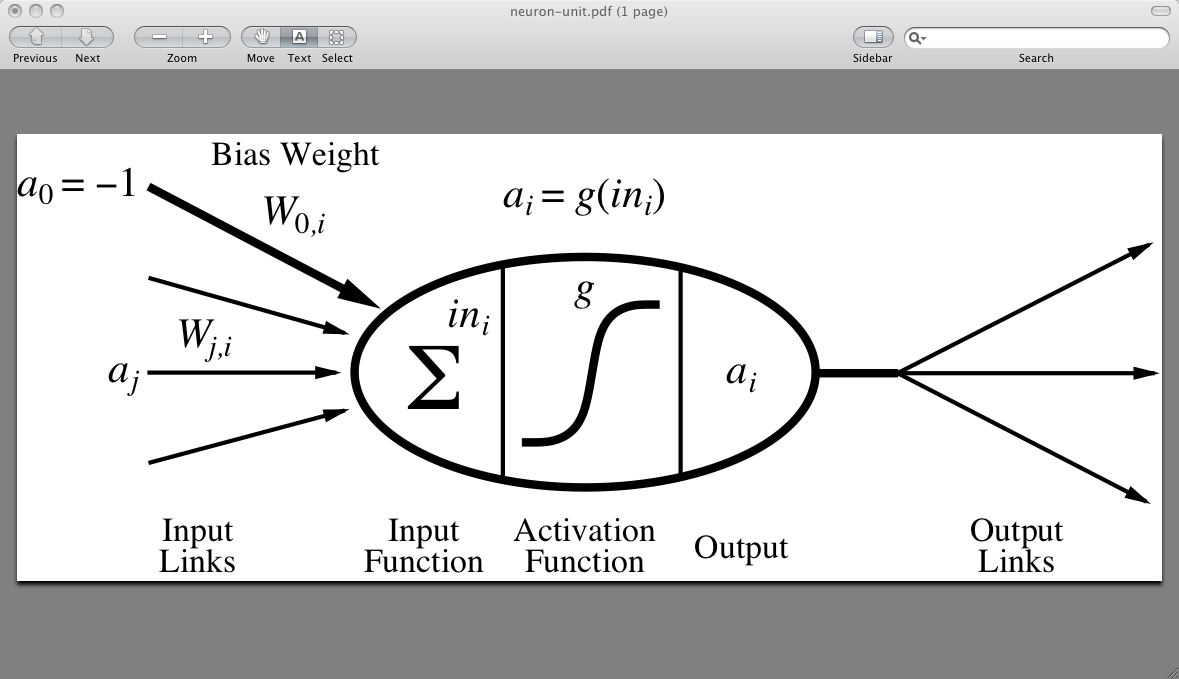
\includegraphics[width=3.5in]{./images/neuron-unit.png}
\end{answer}

\item Figure \ref{fig:nn} shows a backprogation network, with weights as shown and all biases set to 0, that is currently processing the training vector $[1.0, 0.9, 0.9]$ which has an  associated target vector $[0.1, 0.9, 0.1]$. Given that the output from unit B is $0.6$ and from C is $0.8$, and assuming that the activation function used at all nodes in the network is the logistic function (i.e., $f(x) = \frac{1}{1 + \exp^{-x}}$): 
\begin{enumerate}
	\item Calculate the actual output vector (to 3 decimal places).
		\marks{5}
		\begin{answer}
		Output of unit $i = f(\sum_{j=1}^{n}W_{j,i}\times activation_j)$\\
		First output unit input = -0.3 x 0.6 + 0.9 x 0.8 = 0.54 $\rightarrow$ f(0.54) = 0.632\\
		Second output unit input = -0.6 x 0.6 + -0.1 x 0.8 = -0.44 $\rightarrow$ f(-0.44) = 0.392\\
		Third output unit input = 0.4 x 0.6 + 1.2 x 0.8 = 1.2 $\rightarrow$ f(1.2)= 0.769\\
		\end{answer}
	\item Calculate the error for each output unit.
		\marks{5}
		\begin{answer}
		Error =  target - output\\
		First output unit = (0.1 - 0.632)  = - 0.532\\
		Second output unit = (0.9 - 0.392) = 0.508\\
		Third output unit = (0.1 - 0.769) = - 0.669\\
		\end{answer}
	\item Calculate the error for each hidden unit B and C.
		\marks{10}
		\begin{answer}
		Each hidden node $j$ is responsible for some fraction of the error $Err_i$ of each of the output units $i$ to which it connects. Thus the $Err_i$ values are divided according to the strengths of the connection between the hidden node and the output nodes and are propagated back to the hidden nodes. Where a hidden node feeds-forward into more than 1 output node the errors propagated back to it are summed: $Err_j = \sum_{i=1}^{n}W_{ji} \times Err_i$:
		$Err_{B} = (-0.3 \times -0.532) + (-0.6 \times 0.508) + (0.4 \times -0.669) = 0.1596 + -0.3048 + -0.2676 = -0.4128$\\
		$Err_{C} = (0.9 \times -0.532) + (-0.1 \times 0.508) + (1.2 \times -0.669) =  -0.4788 + -0.0508 + -0.8028  = -1.3324$\\
		\end{answer}
\end{enumerate}
\end{enumerate}

\begin{figure}[htbp]
\begin{center}
\includegraphics[width=3.5in]{./images/nn_callan_q10_2.png}
\caption{Example Neural Net}
\label{fig:nn}
\end{center}
\end{figure}


\end{document}
